% CREATED BY DAVID FRISK, 2018
\chapter{Piloto visual con \textit{Deep Learning}}

Introducidos ya todos los elementos de este trabajo, es posible centrarse en el objetivo principal: el desarrollo de un controlador visual basado en \textit{deep learning} para la conducción autónoma de un robot real. En este capítulo se describen todos los elementos del desarrollo de este algoritmo de control visual. Para ello se expondrán los conjuntos de datos utilizados para el entrenamiento del modelo, seguido de los controladores de ROS para los sensores y actuadores del robot real (JetBot) para concluir con la explicación de los detalles de las redes neuronales utilizadas. El capítulo concluye con la validación experimental del modelo construido, en la plataforma BehaviorStudio.

\section{Conjuntos de datos de entrenamiento}
\label{sec:datasets}

Puesto que el algoritmo que se ha desarrollado está basado en aprendizaje supervisado, se necesita un conjunto de datos adecuado sobre los que entrenar el modelo. En aprendizaje automático existen diferentes técnicas de entrenamiento: aprendizaje supervisado, no supervisado, semi-supervisado, auto supervisado y por refuerzo. En este caso se utiliza el aprendizaje supervisado.

En el aprendizaje supervisado se parte de un conocimiento a priori. El modelo trabaja con datos etiquetados, es decir, para una determinada entrada de datos $X$, se espera que el modelo ajuste sus pesos adecuadamente para que le asigne una etiqueta $\hat Y$ a dichos datos de entrada, ajustándose lo máximo posible a la etiqueta proporcionada $Y$. Es mediante la diferencia o error entre la etiqueta $Y$ y la predicción del modelo $\hat Y$ que el algoritmo es capaz de aprender a base de ejemplos. Este tipo de aprendizajes se suele utilizar en problemas de clasificación, donde las etiquetas son categóricas y de regresión donde las etiquetas son numéricas. Usualmente, el reto del aprendizaje supervisado es la obtención de los datos, ya que para que el modelo sea robusto se necesita una gran cantidad de datos etiquetados que tienen que ser representativos y variados; aunque en la práctica, no todos los problemas necesitan una gran cantidad de datos etiquetados, como es el caso de este proyecto.

\begin{figure}
	\begin{center}
		\subfloat[]{\label{fig:original}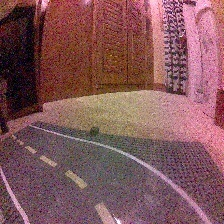
\includegraphics[width=.32\linewidth]{img/original.jpg}}
		\hspace{0.1cm}
		\subfloat[]{\label{fig:sinlinea}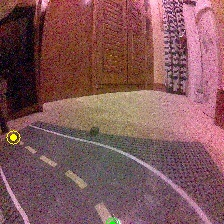
\includegraphics[width=.32\linewidth]{img/sinlinea.jpg}}
		\hspace{0.1cm}
		\subfloat[]{\label{fig:conlinea}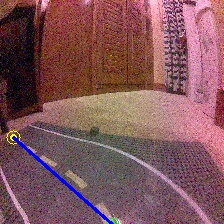
\includegraphics[width=.32\linewidth]{img/conlinea.jpg}}
	\end{center}
	\centering
	\captionsetup{justification=centering,margin=2cm}
	\caption{(a) Imagen captada por el robot, (b) Ejemplo de imagen etiquetada y (c) Ejemplo de imagen etiquetada con información de dirección.}
	\label{fig:dataexample}
\end{figure}

Dado que el problema consiste en realizar un controlador visual para el robot real, los datos de entrada del algoritmo son únicamente imágenes captadas por la cámara a bordo del robot. Como se verá más adelante, se va a enfocar el problema del controlador visual como un problema de regresión donde el modelo ha de predecir las coordenadas $x$ e $y$ de la imagen que mejor aproximen la dirección de movimiento del robot, por lo que estas coordenadas x e y son las etiquetas de las imágenes de entrada, que serán normalizadas antes de entrar al modelo. A partir de las coordenadas $x$ e $y$, se pueden aproximar valores de potencia para comandar a los motores aproximando un ángulo de giro mediante el cálculo del arco tangente entre las coordenadas inferidas por la red. Este valor es posteriormente modulado por un controlador PD y sumado al valor de velocidad lineal obteniendo un valor aproximado de potencia que entregar para cada uno de los motores. La velocidad lineal es constante y se modula para cada experimento.

En la Figura \ref{fig:original}, se puede ver una muestra de lo que el robot <<ve>> a través de la cámara. Un ejemplo de imagen etiquetada con las coordenadas ($x$, $y$) se puede observar en la Figura \ref{fig:sinlinea}, mientras que una intuición de lo que será el comando de actuación del modelo hacia el robot se puede ver en la Figura \ref{fig:conlinea}.

Este conjunto de datos ha sido grabado y etiquetado de forma manual, y consiste en 250 imágenes con resolución 224x224 píxeles, grabadas en diferentes sectores de la pista (rectas, curvas a izquierdas, curvas a derechas, etc.) en diferentes localizaciones con diferente iluminación. Esta variabilidad en la muestra es necesaria para que el modelo sea capaz de generalizar bien ante escenarios que nunca se le han presentado, como otros circuitos u otros entornos diferentes con iluminaciones diversas. En la Figura \ref{fig:variability} se pueden observar algunas muestras de este conjunto de datos y la variabilidad de las mismas.

\begin{figure}
	\begin{center}
		\subfloat{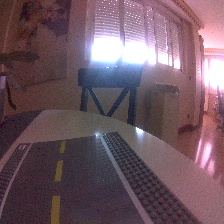
\includegraphics[width=.45\linewidth]{img/recta}}
		\hspace{0.1cm}
		\subfloat{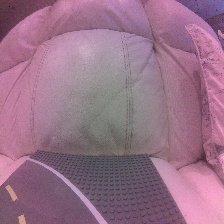
\includegraphics[width=.45\linewidth]{img/cizq}}
		\hspace{0.1cm}
		\subfloat{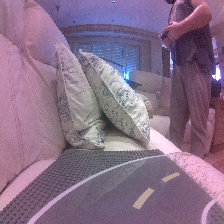
\includegraphics[width=.45\linewidth]{img/cder}}
		\hspace{0.1cm}
		\subfloat{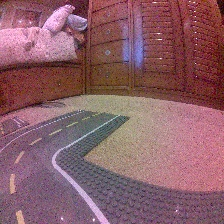
\includegraphics[width=.45\linewidth]{img/sinuoso}}
	\end{center}
	\centering
	\captionsetup{justification=centering,margin=2cm}
	\caption{Ejemplos de algunas muestras del conjunto de datos A}
	\label{fig:variability}
\end{figure}

El preprocesado de las muestras del conjunto de datos antes de entrar al modelo es mínimo, ya que las única transformaciones que se realizan sobre las imágenes son: 

\begin{itemize}
    \item \textbf{Re-escalado} de todas las imágenes de entrada a 224x224 píxeles para que todas las muestras tengan la misma resolución espacial. Se ha seleccionado esta resolución ya que es la que acepta el modelo neuronal que se va a utilizar para resolver el problema. Esto se explica más detalladamente en la sección \ref{sec:regression}.
    \item \textbf{Normalización de la muestra}. La normalización en intensidad aplicada a cada capa de la imagen se realiza a través de la ecuación de la variable estandarizada o normalizada (\textit{z-score} o \textit{default score} en inglés. Esta normalización se define como <<el número de desviaciones típicas que un valor dado toma con respecto a la media de su muestra o población>> según la Wikipedia\footnote{\url{https://es.wikipedia.org/wiki/Unidad_tipificada}}. En este proyecto, se ha normalizado la muestra utilizando esa fórmula con valores de media y desviación típica calculados a partir del conjunto de datos Imagenet, dado que es el conjunto de datos con el que se han pre-entrenado las redes que se han utilizado en este trabajo. La normalización de la muestra ayuda a obtener datos dentro de un rango y reduce el sesgo que mejora y acelera el aprendizaje de los modelos.
    \item \textbf{Modificación del color} (\textit{color jitter}). Para cada muestra se cambia de forma aleatoria el brillo, el contraste y la saturación. Este tipo de transformaciones ayuda a que las redes generalicen mejor, ya que hacen que la muestra sea independiente de los colores concretos que contenga y que el modelo se centre en otro tipo de información, como en este caso, la forma y disposición de las líneas que delimitan la pista.
    \item \textbf{Normalización de las salidas (etiquetas)}. Como se ha comentado más arriba, se ha enfocado este problema como un problema de regresión, por lo que el modelo tendrá que predecir coordenadas en la imagen. Dado que el rango de valores posibles de salida oscila entre 2 órdenes de magnitud (entre 0 y 224) se requiere una normalización de las etiquetas, como técnica de regularización del modelo. Esta normalización previene que algunos pesos de la red se disparen con respecto a otros porque los valores de las etiquetas normalizadas estarán contenidos en rangos más estándar (típicamente entre 0 y 1, o entre -1 y 1), ayudando a que no se produzca el problema de la explosión de gradientes, además de ayudar en la convergencia.
\end{itemize}

La forma en la que Pytorch realiza estas transformaciones se aplica en la construcción de cada mini-lote (o \textit{mini-batch} en inglés). Esto quiere decir que en cada iteración durante el entrenamiento, Pytorch extraerá copias de las muestras del conjunto de datos de entrada original (sin adulterar), realizará las transformaciones fijas (como el re-escalado y la normalización, y las transformaciones aleatorias como los cambios en los niveles de brillo, contraste y saturación (\textit{color jitter}). Este carácter aleatorio de las transformaciones, hace de éstas una técnica de aumento de datos, ya que se aplican en cada iteración durante el entrenamiento por lo que en cada época, estas transformaciones pueden ser diferentes ante la misma muestra de entrada.

Adicionalmente al conjunto de datos de 250 imágenes con gran variabilidad, se ha grabado otro conjunto aún mayor para tratar de experimentar con diferentes conjuntos de datos. Este nuevo conjunto de datos consta de 550 imágenes con las mismas propiedades que el conjunto de datos principal, pero con la única diferencia de que está sesgado. Todas las imágenes de este nuevo conjunto de datos están grabadas en el mismo escenario (la misma habitación), con una iluminación relativamente uniforme. La Figura \ref{fig:dataexample}, contiene tres muestras de este conjunto de datos. Todos los conjuntos de datos tienen las mismas propiedades y se le realizan las mismas transformaciones. En resumen, se dispone de 2 conjuntos de datos diferentes:

\begin{itemize}
    \item \textbf{Conjunto de datos A}. Compuesto de 250 imágenes variadas en cuanto a iluminación, y entornos, de diferentes tramos de la pista. Este conjunto de datos está balanceado con respecto a los diferentes tipos de tramos: rectas, curvas a izquierda y curvas a derecha. También está balanceado en cuanto a variabilidad de fondos y de iluminación.
    \item \textbf{Conjunto de datos B}. Compuesto de 550 imágenes con iluminación y fondos similares. Está balanceado en cuanto a tipos de tramos de la pista: rectas, curvas a izquierda y curvas a derecha, pero está sesgado en cuanto a variabilidad en iluminación y fondos.
\end{itemize}

\section{\textit{Drivers} JetBot}

Para poder conectar el \textit{hardware} del robot con la plataforma BehaviorStudio y los diferentes cerebros neuronales que gobernarán al mismo, es necesario un mecasnimo de comunicación entre ambas partes. En el caso del robot simulado, los propios modelos y la propia infraestructura de JdeRobot incluía resueltas esas conexiones, al implementar cada sensor y actuador del robot interfaces de comunicación a través de \textit{topics} de ROS. No obstante, no se dispone de esa facilidad en el caso del robot real. Por este motivo, se ha desarrollado un controlador capaz de conectar los sensores del robot JetBot (la cámara) y los actuadores del mismo (los motores) basado también en \textit{topics} de ROS para habilitar la comunicación entre el robot y la plataforma BehaviorStudio.

\begin{figure}
  \centering
  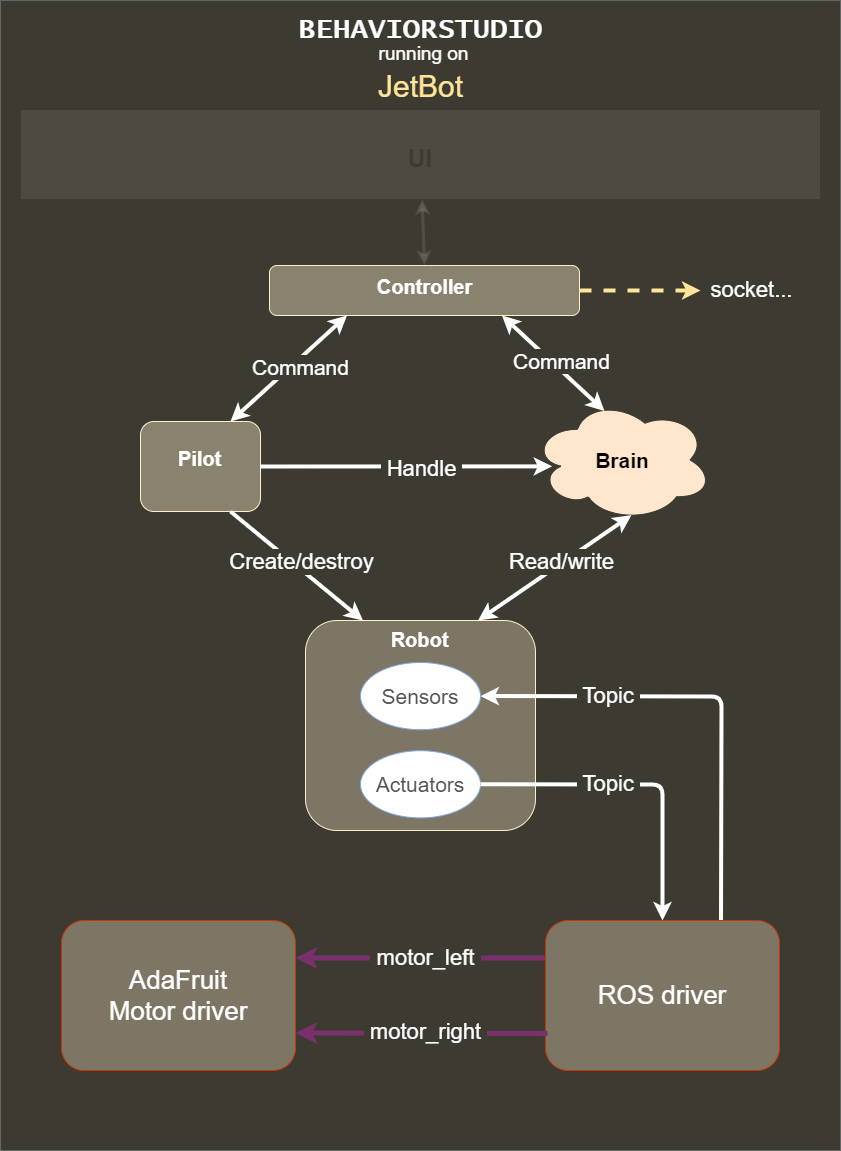
\includegraphics[width=.8\linewidth]{img/rosdriver.png}
  \caption{Arquitectura de BehaviorStudio corriendo en el robot JetBot}
  \label{fig:rosdriver}
\end{figure}

La imagen que sirve como sistema operativo del robot, que se ha utilizado (JetPack 4.3) dispone de un API en Python para acceder a todos los elementos del robot: cámara, motores, pantalla OLED, batería, etc. Se ha desarrollado un envoltorio que encapsula esa funcionalidad recubriéndola con lógica de \textit{topics} de ROS, de tal forma que se han creado interfaces para la cámara y los motores. Este desarrollo se ha inspirado en un envoltorio ya existente del JetBot para ROS\footnote{\url{https://github.com/dusty-nv/jetbot_ros}}, que resuelve el problema de las comunicaciones. No obstante, después de las pruebas realizadas sobre este código se comprobó que las interfaces no funcionaban del todo bien, ya que la imagen de la cámara se obtenía rotada 180 grados y el movimiento de los motores no funcionaba bien en ocasiones. Por este motivo se optó por desarrollar un híbrido entre el código del \textit{driver} de ROS existente para el JetBot y los \textit{drivers} que ofrece la propia imagen JetPack del robot, obteniendo una iteración sobre las dos APIs con pequeños cambios que solucionaban los problemas mencionados. En la Figura \ref{fig:rosdriver} se puede apreciar un diagrama de la arquitectura de este componente.

Los \textit{topics} asociados a cada sensor/actuador son similares a los utilizados en el robot simulado. Para la cámara, el \textit{topic} utilizado transporta el mismo tipo de mensajes que para el robot real (\texttt{std\_msgs/Image}) mientras que para los comandos de velocidad lineal y angular de los motores del robot se utilizan mensajes de tipo Float32 de ROS (\texttt{std\_msgs/Float32.msg}).

Este controlador se ejecuta mediante \textit{scripts} de Python, de tal forma que se pueda automatizar el lanzamiento de los algoritmos mediante el cron de Linux o convirtiéndolos en servicios del sistema para que estén siempre operativos. Una vez funcionando, la conexión con la plataforma es directa, ya que está preparada para aceptar conexiones mediante \textit{sockets} utilizando ROS, al igual que el entorno de simulación.

\section{Redes de regresión para control visual de un robot}
\label{sec:regression}

Muchas redes neuronales son usadas típicamente para resolver tareas de detección y clasificación. En visión artificial las redes neuronales convolucionales de detección son las más conocidas; arquitecturas como la YOLO que han demostrado ser muy potentes para la clasificación de objetos en imágenes, se utiliza en multitud de trabajos de visión en la comunidad investigadora e incluso en las empresas. No obstante, las redes neuronales también son muy útiles en problemas de regresión. El problema de la regresión consiste en predecir el valor de una variable continua en función del valor de otras variables independientes.

En el caso de las redes neuronales, la regresión se aplica en problemas en los que las variables a predecir no pueden ser categorizadas en diferentes clases; el espacio de posibles predicciones no es discreto. Se considera que la regresión es un problema de clasificación de infinitas clases, ya que trata de modelar la relación existente entre una variable continua (dependiente) que se trata de predecir, en base a otras variables (independientes) que son las entradas al modelo.

Las redes neuronales de regresión en visión artificial se suelen utilizar para solucionar problemas de segmentación a nivel de píxel, estimación de \textit{bounding boxes} en una imagen, detección de pose humana, etc. En este trabajo se utiliza la regresión para estimar las coordenadas $XY$ a las que el robot debería estar mirando, de tal forma que si el robot está desviado de su trayectoria en una curva o una recta, se corrija su posición mediante la inferencia. Es decir, se predicen las coordenadas de la imagen donde se supone que el robot debería dirigirse. Estos valores están directamente relacionadas con las velocidades de avance $v$ y de giro $w$ que se van a ordenar a los motores.

La resolución del problema se basa en alimentar a la red con las imágenes captadas por el robot en cada momento, de tal forma que se infieran las coordenadas $XY$ de la imagen que representa la dirección a la que se debe mover el robot. Como se comentó en secciones anteriores, las etiquetas de los datos ha sido normalizadas a valores entre -1 y 1, por lo que el modelo inferirá las coordenadas con esa normalización. A partir de dichas coordenadas se aproximará un ángulo de giro mediante el cálculo de la arcotangente con signo entre ambas coordenadas de la inferencia. Este ángulo será corregido mediante un controlador PD (Proporcional-Derivativo), para dotar al movimiento de suavidad y que no sea tan reactivo ante cambios. Además a la ecuación se suma el sesgo de las ganancias de los motores, para corregir desviaciones en la trayectoria naturaleza de la limitación de los motores. La ecuación resultante es:

$$
pd\_val = angle * kp + (angle - angle_last) * kd
$$

\noindent aplicando la correción del sesgo:

$$
steer = pd\_val + steer\_bias
$$

\noindent aplicando una fuerza final a cada motor resultado de la suma de la velocidad lineal y la velocidad angular calculada en las ecuaciones anteriores con límites entre 0 y 1, de modo que si el valor agregado de velocidad lineal y angular supera el umbral por encima o por debajo, se apliquen los valores máximo o mínimo respectivamente.

Para solucionar el problema se han seleccionado dos tipos de arquitecturas de redes neuronales, una basada en redes residuales y otra basada en redes convolucionales convencionales: ResNet y MobileNet respectivamente. En las siguientes secciones se ofrece una descripción breve de ambas arquitecturas.

\subsection{Arquitectura ResNet}
\label{sec:resnet}

La arquitectura ResNet surgió en 2015 \cite{resnet} con la idea de solucionar el problema que sufrían todas las redes de clasificación del momento, que consistía en que las repuestas se degradaban exponencialmente al aumentar la profundidad de las redes neuronales, el conocido <<desvanecimeinto del gradiente>>. El problema se solucionó con la inclusión de determinadas conexiones que <<saltaban>> capas de las redes tradicionales, permitiendo aumentar el número de capas sin que el rendimiento de la red se viera afectado, y solucionando así el problema del desvanecimiento del gradiente. Estas conexiones fueron implementadas mediante <<bloques residuales>> formados esencialmente de dos capas convolucionales y una conexión que suma la salida de esas capas y la entrada, como se aprecia en la Figura \ref{fig:residualblock}

\begin{figure}
  \centering
  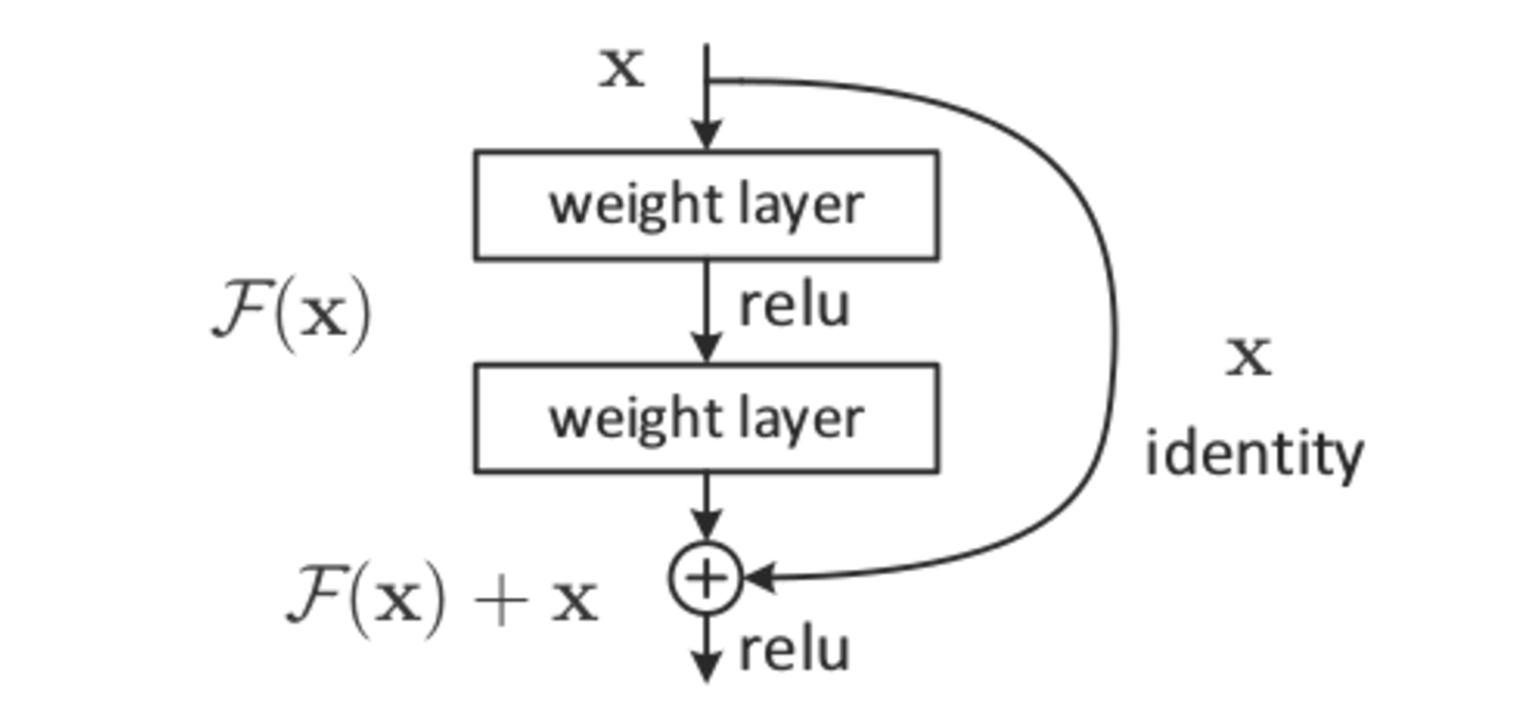
\includegraphics[width=1\linewidth]{img/residualblock.png}
  \caption{Bloque residual de la arquitectura ResNet.}
  \label{fig:residualblock}
\end{figure}

Existen numerosas variantes de esta arquitectura con diferentes número de capas, desde 18 hasta 152. En este trabajo se exploran dos de ellas: la arquitectura ResNet-18 y la arquitectura ResNet-34. Estas arquitecturas se muestran en la Figura \ref{fig:resnets}

\begin{figure}
	\begin{center}
		\subfloat{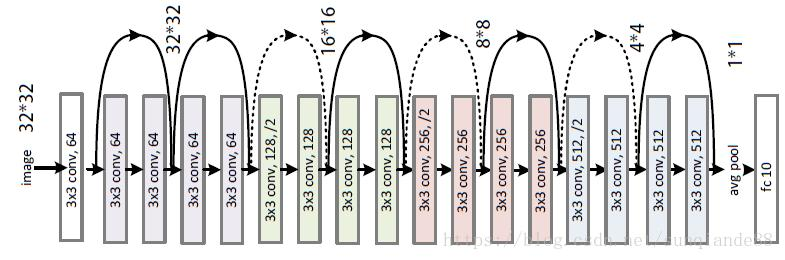
\includegraphics[width=1\linewidth]{img/resnet18}}
		\hspace{0.1cm}
		\subfloat{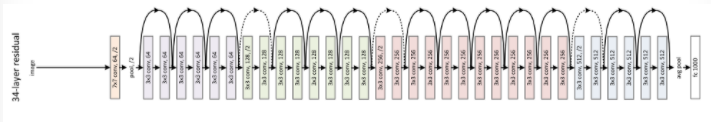
\includegraphics[width=1\linewidth]{img/resnet34}}
	\end{center}
	\centering
	\captionsetup{justification=centering,margin=2cm}
	\caption{Arquitecturas ResNet-18 (arriba) y ReNet-34 (abajo)}
	\label{fig:resnets}
\end{figure}

Pytorch ofrece multitud de redes pre-entrenadas\footnote{\url{https://pytorch.org/docs/stable/torchvision/models.html}} que están listas para ser utilizadas sin necesidad de un ajuste fino si no se requiere. Estos modelos pueden ser instanciados a través de la biblioteca \texttt{torchvision} que está dedicada a la visión artificial. En concreto, las redes utilizadas en este trabajo (la ResNet-18 y la ResNet-34) están pre-entrenadas con el conjunto de datos ImageNet para la tarea de clasificación de imágenes. Dado que se va a abordar el problema de la conducción autónoma como una tarea de regresión, es necesario hacer una transferencia de dominio del conocimiento de estas redes, de tal forma que aprendan a realizar inferencia sobre nuestro problema en concreto. La forma de instanciar estos modelos pre-entrenados es posible a través del API de la biblioteca \texttt{torchvision} como muestra el Fragmento \ref{resfragment}

\begin{tabular}{c}
\begin{lstlisting}[caption={Ejemplo de instanciación de diferentes modelos pre-entrenados.},captionpos=b,label=resfragment,style=Python] 
import torchvision

# instancia de una ResNet-18 pre-entrenada
model = torchvision.models.resnet18(pretrained=True)

# instancia de una ResNet-34 pre-entrenada
model = torchvision.models.resnet34(pretrained=True)

# instancia de una red MobileNet v2
model = torchvision.models.mobilenet_v2(pretrained=True)

\end{lstlisting}
\end{tabular}

\subsection{Arquitectura MobileNet}
\label{sec:mobilenet}

Los modelos basados en redes neuronales más grandes y potentes requieren de una potencia de cómputo altísima tanto para entrenar como para realizar inferencias. No obstante, en los últimos años han surgido modelos basados en redes neuronales que están diseñados para funcionar en dispositivos móviles y de recursos limitados como los los sistemas embebidos. Este es el caso de MobileNet.

Para conseguir esto, Mobilenet utiliza los llamados bloques \textit{bottleneck}, que se pueden observar en la Figura \ref{fig:mobileblock}. Este bloque básicamente realiza una factorización sobre la convolución normal separándola en varias capas. La primera capa llamada \textit{depthwise convolution} aplica un único filtro por canal de la imagen, posible al ser precedido por una convolución 1x1 previamente. La capa siguiente recibe el nombre de \textit{pointwise convolution} y se encarga de crear características nuevas en base a la combinación lineal de los canales de entrada de la imagen.

\begin{figure}
  \centering
  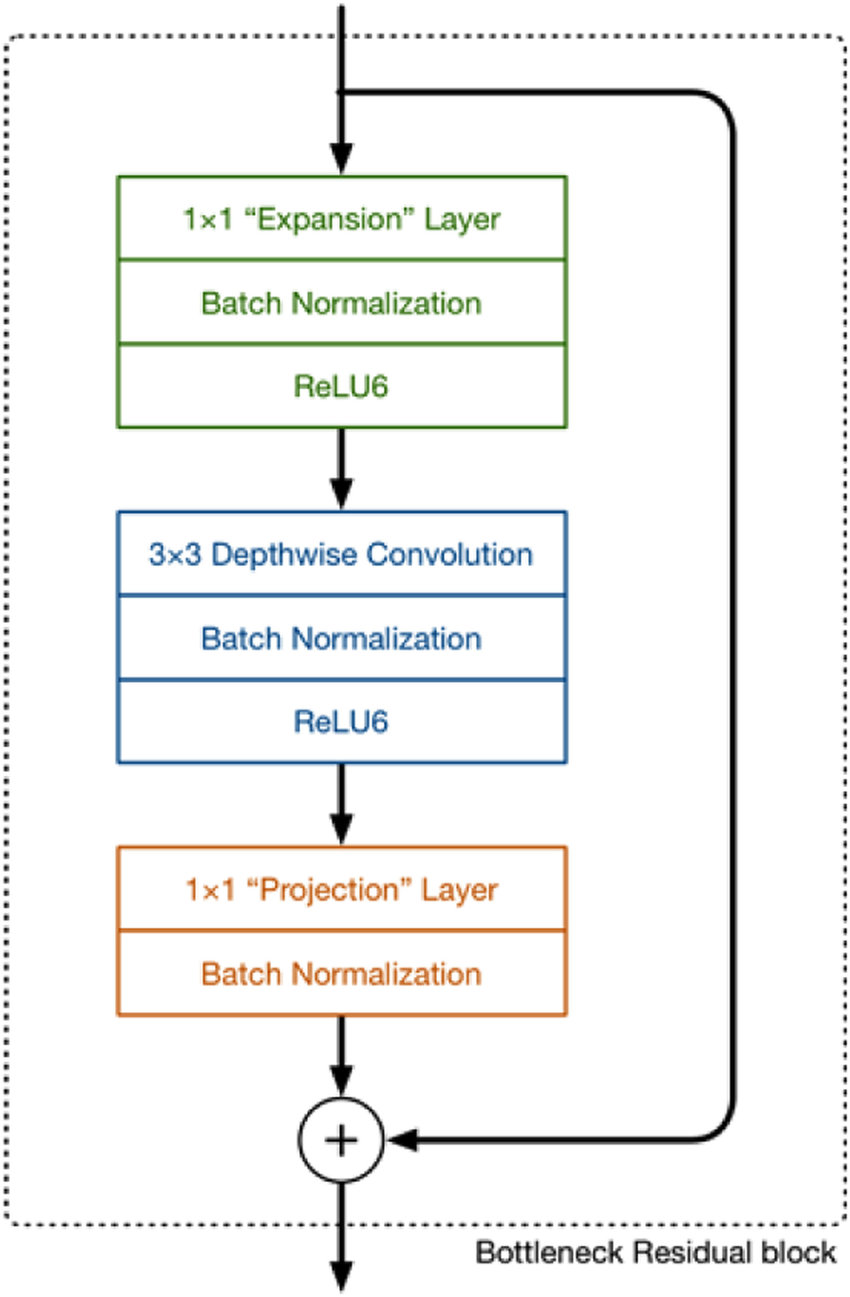
\includegraphics[width=.4\linewidth]{img/mobileblock.jpg}
  \caption{Bloque residual \textit{bottleneck} de la arquitectura MobileNet v2.}
  \label{fig:mobileblock}
\end{figure}

Al igual que con las arquitecturas ResNet, Pytorch ofrece también la arquitectura MobileNet v2. Esta red también está pre-entrenada con el conjunto de datos ImageNet para la clasificación de imágenes, lista para ser utilizada. Esta arquitectura está disponible en el mismo sitio que las ResNet mencionadas en arriba y se instancia como se muestra en el Fragmento \ref{resfragment}.

\section{\textit{Transfer Learning}}
\label{sec:transfer}

Una técnica que se puede aplicar en el \textit{deep learning} es la transferencia de aprendizaje, comúnmente conocida como \textit{transfer learning}. La técnica de \textit{transfer learning} consiste en seleccionar una red neuronal ya entrenada con un conjunto de datos determinado y usarla como punto de partida para que la red aprenda a desarrollar otra tarea diferente. Por ejemplo, se puede tomar un modelo neuronal sin entrenar como la ResNet-18, entrenarla con un conjunto de datos para una tarea concreta (ImageNet para clasificación de imágenes, por ejemplo) obteniendo una red entrenada, a la que denominaremos ResNet-18 en este ejemplo, para dicha tarea. Durante el proceso de aprendizaje, ResNet-18 habrá aprendido un amplio conjunto de filtros de características que pueden ser reutilizadas para tareas parecidas, por lo que en este momento se puede partir de esa red pre-entrenada para que aprenda a realizar otra tarea (como la de la estimación de coordenadas en una imagen) con otro conjunto de datos diferente que con los que fue pre-entrenada. El modelo resultante sobre el que se ha aplicado \textit{transfer learning} se distingue en este documento con un asterisco <<*>>, de tal forma que en este ejemplo concreto el modelo re-entrenado se denominará ResNet-18*. Esta técnica otorga mejoras significativas en el proceso de aprendizaje, ya que entre otras cosas requiere menos ajuste de hiperparámetros, ayuda a la convergencia, está validado el buen rendimiento de la arquitectura de antemano y suele requerir un entrenamiento menos exhaustivo.

Para entrenar los modelos seleccionados para este trabajo, se ha aplicado \textit{transfer learning} por los motivos expuestos más arriba. A pesar de que los modelos están ya entrenados con un dominio específico, en este caso con el conjunto de datos de ImageNet, es necesario que aprenda a resolver la tarea de la conducción autónoma, por lo que hay que reentrenar los 3 modelos con un conjunto de datos del problema concreto a resolver. Este reentrenamiento requiere primero de unos datos concretos (se describieron en la sección \ref{sec:datasets}) y segundo de un ajuste de algunos hiperparámetros como el tamaño de los lotes que van a entrar al modelo, el número de épocas de entrenamiento o el porcentaje de datos que se usarán para entrenar y validar el modelo. Durante el desarrollo de el trabajo se han probado diferentes configuraciones sobre el circuito de pruebas (el circuito \textit{Training} que se introduce en la siguiente sección). Dado que se ha aplicado \textit{transfer learning}, los únicos parámetros que se han modificado han sido los necesarios para el reentrenamiento: el número de épocas de entrenamiento, el tamaño del mini-lote, el optimizador y la proporción en los conjuntos de datos de entrenamiento y de pruebas. Para los 3 modelos entrenados se han definido los mismos parámetros, por simplicidad: 70 épocas de entrenamiento, tamaño de mini-lote de 8, optimizador Adam con parámetros por defecto y una proporción de los conjuntos de entrenamiento-test de 80-20 (80\% de los datos utilizados para el entrenamiento y el 20\% restante para test).

El segundo experimento realizado se ha llevado a cabo mediante el entrenamiento de una red ResNet-18. Como se explicó en la sección \ref{sec:resnet}, las redes residuales que ofrece Pytorch han sido entrenadas con el conjunto de datos de ImageNet, por lo que se ha aplicado la técnica de \textit{transfer learning}. Se ha demostrado que esta técnica aumenta de forma considerable el rendimiento de las redes a nivel de inferencia ya que han sido pre-entrenadas con conjuntos de datos muy grandes y muy bien construidos, por lo que los filtros que se aprendieron durante ese entrenamiento aportan un conocimiento a priori que se aprovecha al realizar el cambio de dominio. Las arquitecturas ResNet que ofrece Pytorch pre-entrenadas varían desde las 18 capas hasta las 152. Para este proyecto se ha utilizado la red más pequeña, la ResNet-18, que proporciona un buen equilibrio de rendimiento y eficiencia para la Jetson Nano.

Tras los reentrenamientos respectivos se obtuvieron sendas redes de regresión: ResNet-18*, ResNet-34* y MobileNet-v2* ya adaptadas a la conducción automática del robot JetBot.


\subsection{Métricas de evaluación de los entrenamientos}
\label{sec:metrics}

Es necesario definir algún tipo de métrica para evaluar cómo de bien o de mal han ido los entrenamientos de las diferentes redes de regresión. En este caso, las métricas más típicas de validación que se utilizan para este tipo de redes son las de el error cuadrático medio (MSE o \textit{Mean Squared Error} por sus siglas en inglés) y el error absoluto medio (MAE o \textit{Mean Absolut Error} por sus siglas en inglés). Este tipo de métricas se calculan mediante la diferencia entre las etiquetas de los datos y las predicciones de la red.

La métrica MAE se calcula como el promedio de la diferencia entre los valores de las etiquetas y los valores predichos por la red ante una entrada determinada. Esta medida ayuda a determinar cómo de diferentes son estos dos valores, ya que un error alto indica que la red no se está acercando al valor real que se espera (la diferencia es mayor), mientras que un error bajo indica que las predicciones de la red y los valores reales se parecen. No obstante, esta métrica no aporta información sobre la dirección del error, por lo que no se puede determinar si el error es provocado por predicciones que estén por encima o por debajo del valor de la etiqueta. La ecuación matemática del MAE se expresa como sigue:

$$MAE=\frac{1}{N}\sum_{i=1}^{N}|y_i-\hat y_i|$$

Donde N es el número total de muestras a entrenar, $y_i$ es el valor de la etiqueta de la muestra $i$-ésima, e $\hat y_i$ es el valor predicho por la red para la muestra $i$-ésima.

Por otra parte, la métrica MSE se calcula como el promedio del cuadrado de la diferencia entre los valores de las etiquetas y los valores predichos por la red. Las métricas son muy similares, pero la ventaja de MSE sobre MAE es que el primero facilita el cálculo del gradiente. Esto es así ya que los fallos en las predicciones penalizan mucho más al calcular el cuadrado del error, por lo que la diferencia entre errores grandes y errores pequeños es más pronunciada. La ecuación matemática del MSE se calcula como sigue:

$$MSE=\frac{1}{N}\sum_{i=1}^{N}(y_i-\hat y_i)^2$$

Donde, al igual que para MAE, N es el número total de muestras a entrenar, $y_i$ es el valor de la etiqueta de la muestra $i$-ésima, e $\hat y_i$ es el valor predicho por la red para la muestra $i$-ésima.

Tanto MAE como MSE ayudan a determinar cómo de bien ha ido el entrenamiento de las redes neuronales. Este tipo de métricas de entrenamiento son muy útiles para determinar si las redes tienen algún problema como capacidad de aprendizaje, sobreajuste, subajuste, etc. Teniendo un diagnóstico en tiempo real del entrenamiento es posible implementar técnicas como la parada temprana (\textit{Early stopping}), la planificación de la tasa de aprendizaje (\textit{scheduler}), entre otras, que ayudan a una detección temprana de problemas en las redes, dado que, por norma general, las redes neuronales profundas requieren grandes tiempos de entrenamiento. En la Tabla \ref{tab:mae_mse} se recoge las métricas promedio de las redes reentrenadas: Resnet18, ResNet-34 y MobileNet v2.

\begin{table}[ht!]
\ttfamily\small
\centering
\begin{tabular}{|l|c|c|}
\hline
\rowcolor[HTML]{C0C0C0} 
\textbf{Red}                         & \textit{\textbf{Mean Absolute Error}} & \textit{\textbf{Mean Squared Error}} \\ \hline
\cellcolor[HTML]{EFEFEF}Resnet-18    &          0.538007                                  &              0.098720                             \\ \hline
\cellcolor[HTML]{EFEFEF}Resnet-34    &          0.627700                                  &              0.369343                             \\ \hline
\cellcolor[HTML]{EFEFEF}MobileNet v2 &          0.594553                                  &              0.259610                             \\ \hline
\end{tabular}
\caption{Promedio de las métricas de entrenamiento para las redes utilizadas.}
\label{tab:mae_mse}
\end{table}


Es posible que aunque una red arroje buenas métricas de evaluación en el entrenamiento, no se refleje en un buen comportamiento del robot real con ella. Es decir, se puede dar el caso de que a pesar de que las métricas de entrenamiento resulten prometedoras, la ejecución real no sea capaz de solucionar el problema para el que fue entrenada provocando que el robot no sea capaz de completar el circuito. Este es el caso de la red Resnet-34, que aunque arroje resultados similares al resto de las redes probadas, no ha sido capaz de completar ningún circuito. Esto se debe a que el cálculo del error se hace de forma promedio, de tal forma que algunas predicciones pueden ser muy buenas, pero otras pueden ser muy malas, lo que se camufla al realizar la media. Por eso estas métricas pueden dar falsa sensación de éxito. No obstante, en este caso concreto, el problema ha sido el tamaño de la red. La red ResNet-34 es casi el doble de grande que la ResNet-18. Se ha comprobado experimentalmente que la ResNet-18 pone casi al límite las capacidades de la Jetson Nano en cuanto a recursos de CPU y memoria, por lo que la razón principal por las que la ResNet-34 no ha podido completar ningún circuito es por la latencia introducida en cada iteración para obtener una inferencia (llegando a tardar casi 1 segundo en tomar una decisión en cada iteración que es un retardo inaceptable en nua aplicación de control robótico).

Las métricas de validación explicadas dan buenas pistas sobre cómo ajustar los parámetros de entrenamiento. En las Figuras \ref{fig:graficas} se pueden observar los valores de estas métricas en el proceso de reentrenamiento en las diferentes redes. La Tabla \ref{tab:mae_mse}, muestra el promedio de esas métricas para las 70 épocas de reentrenamiento.

\begin{figure}
	\begin{center}
		\subfloat[MobileNet v2]{\label{fig:mbplot}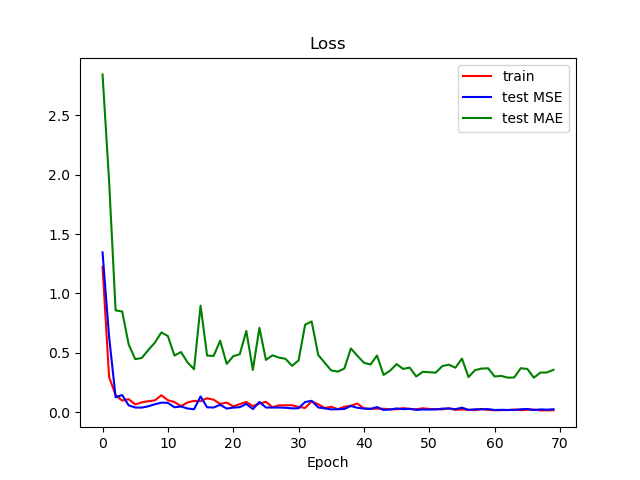
\includegraphics[width=.6\linewidth]{img/training_result_xy_mobilenet_loss.png}}
		\hspace{0.1cm}
		\subfloat[ResNet-18]{\label{fig:r18plot}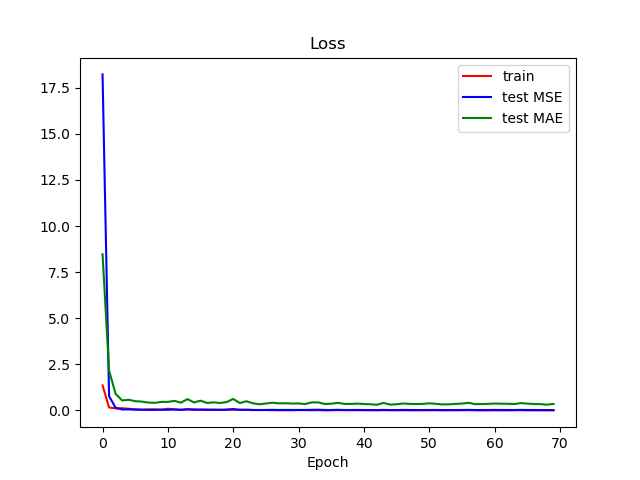
\includegraphics[width=.6\linewidth]{img/training_result_xy_resnet18_loss.png}}
		\hspace{0.1cm}
		\subfloat[ResNet-34]{\label{fig:r34plot}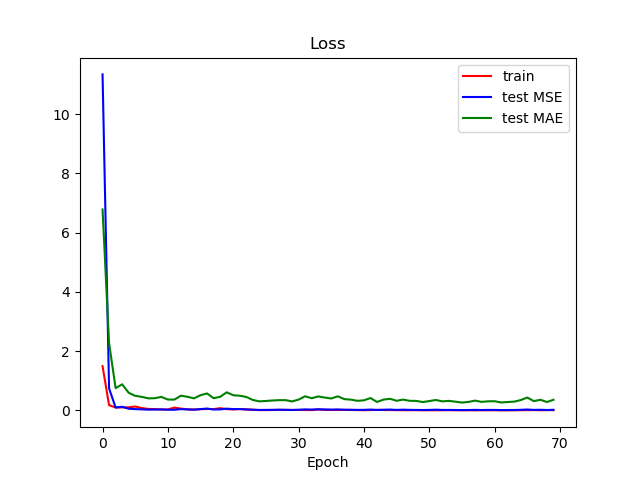
\includegraphics[width=.6\linewidth]{img/training_result_xy_resnet34_loss.png}}
	\end{center}
	\centering
	\captionsetup{justification=centering,margin=2cm}
	\caption{Métricas de pérdida en entrenamiento en 70 épocas de las diferentes redes utilizadas.}
	\label{fig:graficas}
\end{figure}

Como se puede observar, las redes ResNet convergen muy pronto (en torno a las 4 épocas), mientras que MobileNet oscila algo más. No obstante, la pérdida en los tres casos es muy baja, por lo que el error cometido es poco. Esto indica que los parámetros de entrenamiento están bien ajustados. Además, al haber aplicado la técnica de \textit{transfer learning}, el entrenamiento es más rápido y más eficiente. En este caso concreto, se podría haber implementado una parada prematura del entrenamiento, ya que en el caso de las ResNet, a partir de la época 4-5 no se mejora más al estar el error ya muy cercano a cero. En el caso de MobileNet, el entrenamiento no se estabiliza hasta la época 50 aproximadamente. Esto se debe a que el modelo es más pequeño y no generaliza tan bien como los dos anteriores a pesar de haber aplicado \textit{transfer learning} igualmente. No obstante, se ha conseguido que el entrenamiento sea exitoso al no haberse producido ningún problema de subajuste o sobreajuste. 

En la siguiente sección se validará el desempeño de los modelos reentrenados para resolver la tarea en entornos reales. Se obvia la inclusión de la red ResNet-34 ya que no ha conseguido completar ningún circuito debido a problemas de rendimiento con la placa Jetson Nano.


\section{Validación experimental}

Una vez reentrenados los modelos neuronales del controlador visual como se ha explicado en las secciones anteriores, en esta sección se explican los experimentos que validan el trabajo realizado. Como se explicó en el capítulo de introducción, el objetivo es que un robot real sea capaz de completar vueltas a un circuito, o varios en este caso, utilizando como algoritmo de control los modelos neuronales basados en \textit{deep learning} conseguidos. A continuación se describen los diferentes circuitos sobre los que se ha validado el trabajo, las métricas de evaluación utilizadas para validar el correcto funcionamiento de los modelos, los experimentos realizados y los resultados de dichos experimentos.

En la sección \ref{sec:metrics} se explicaron las métricas que se utilizan para validar el entrenamiento de los modelos. No obstante, aún falta definir algún tipo de métrica operativa, que refleje la realidad del aprendizaje conseguido, es decir, poner a prueba las capacidades de la red aprendida. Para ello se define una métrica operativa que será el tiempo que tarda el robot en completar una vuelta al circuito; de este modo, sabremos cómo se comportan las redes entrenadas en ejecución.

\subsection{Circuitos de test}

Para validar que el robot puede solucionar la tarea de la conducción autónoma, es necesario algún tipo de carretera que seguir. Para este propósito se han diseñado diferentes circuitos pequeños a partir de piezas de Lego, como se apuntó en la introducción (Figura \ref{fig:legos}). En concreto se han diseñado 12 circuitos diferentes con configuraciones variadas de curvas y rectas. La longitud de cada segmento recto mide 25 $cm$, mientras que las curvas tienen una longitud de unos 20 $cm$ aproximadamente. Todos los segmentos rectos son exactamente iguales, al igual que ocurre con los segmentos curvos. En la Figura \ref{fig:pistas}, se pueden observar los circuitos propuestos.

\begin{figure}
  \makebox[\textwidth][c]{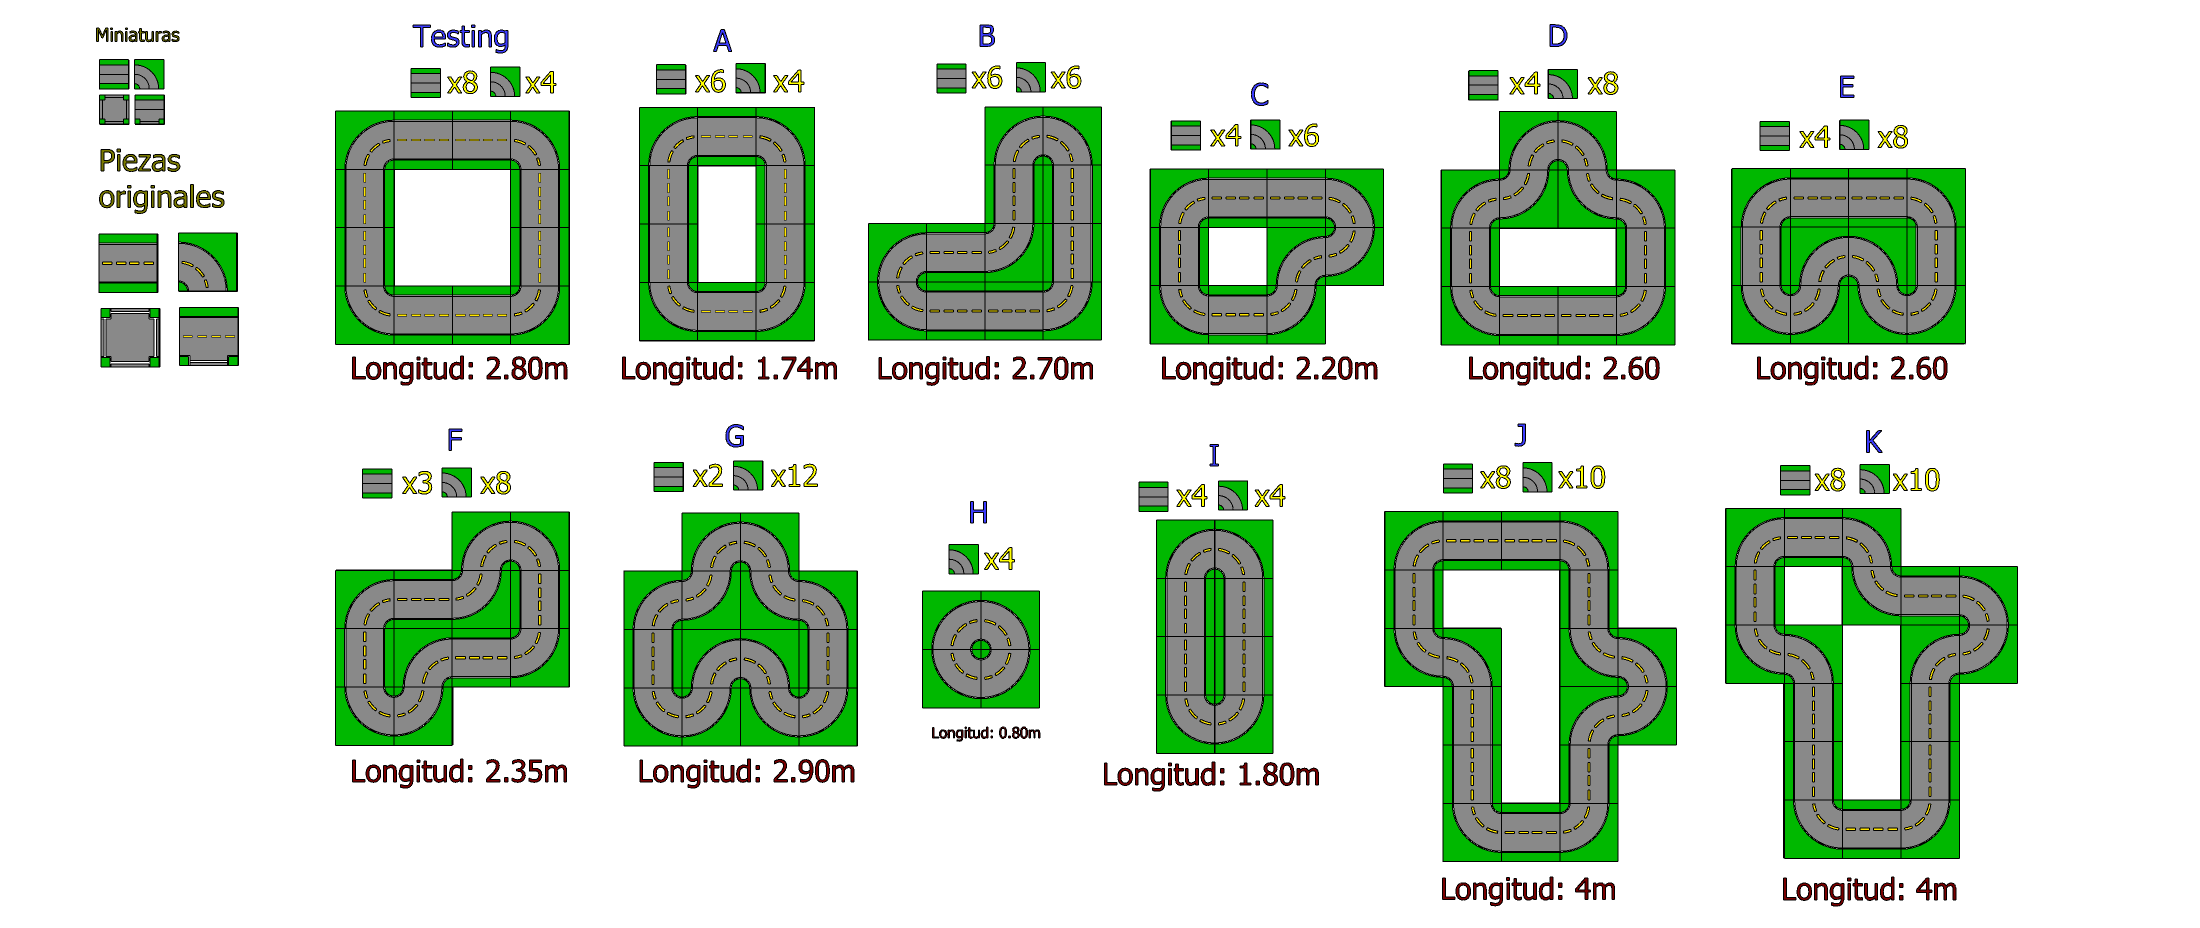
\includegraphics[width=1.3\textwidth]{img/circuits5.png}}%
  \caption{Diferentes circuitos a resolver por el robot.}
  \label{fig:pistas}
\end{figure}

\begin{table}[ht!]
\centering
\ttfamily\tiny
\resizebox{\textwidth}{!}{%
\begin{tabular}{|
>{\columncolor[HTML]{EFEFEF}}c |c|c|c|}
\hline
\cellcolor[HTML]{C0C0C0}\textbf{Circuito} & \cellcolor[HTML]{C0C0C0}\textbf{Longitud (metros)} & \cellcolor[HTML]{C0C0C0}\textbf{\# Rectas} & \cellcolor[HTML]{C0C0C0}\textbf{\# Curvas} \\ \hline
\textbf{Training}                         & 2.80                                               & 8                                          & 4                                          \\ \hline
\textbf{A}                                & 1.74                                               & 6                                          & 4                                          \\ \hline
\textbf{B}                                & 2.70                                               & 6                                          & 6                                          \\ \hline
\textbf{C}                                & 2.20                                               & 4                                          & 6                                          \\ \hline
\textbf{D}                                & 2.60                                               & 4                                          & 8                                          \\ \hline
\textbf{E}                                & 2.60                                               & 4                                          & 8                                          \\ \hline
\textbf{F}                                & 2.35                                               & 3                                          & 8                                          \\ \hline
\textbf{G}                                & 2.90                                               & 2                                          & 12                                         \\ \hline
\textbf{H}                                & 0.80                                               & -                                          & 4                                          \\ \hline
\textbf{I}                                & 1.80                                               & 4                                          & 4                                          \\ \hline
\textbf{J}                                & 4.00                                               & 8                                          & 10                                         \\ \hline
\textbf{K}                                & 4.00                                               & 8                                          & 10                                         \\ \hline
\end{tabular}%
}
\caption{Propiedades de los 12 circuitos propuestos.}
\label{tab:pistas}
\end{table}

Como se puede observar, cada circuito tiene un número diferente de curvas y rectas dispuestos de menor a mayor dificultad, de tal forma que se pueda evaluar la robustez de los modelos entrenados ante circuitos nunca vistos. En las secciones de ejecución típica se muestran los resultados en cuanto a tiempo por vuelta de cada uno de los circuitos propuestos. La Tabla \ref{tab:pistas} muestra un resumen de las características de cada uno de los circuitos. El circuito de \textit{Training} recibe ese nombre ya que es en ese circuito en el que se probaron los modelos hasta conseguir el ajuste óptimo de los hiper-parámetros de las redes.

La evaluación realizada consiste en que el robot sea capaz de completar una vuelta a cada uno de los circuitos en sentido horario y en sentido antihorario. Esto ha de aplicarse a cada uno de los dos modelos reentrenados: Resnet18* y MobileNet-v2*.

\subsection{Ejecución típica MobileNet-v2*}

En este primer experimento se ha hecho uso de una arquitectura MobileNet v2 para entrenar una red con los conjuntos de datos disponibles. Como se explicó en la sección \ref{sec:mobilenet}, este tipo de arquitectura está diseñada para ser implementadas en dispositivos pequeños, como placas de procesamiento tipo RaspberryPi, Serie Jetson y dispositivos móviles. Este ha sido el motivo por el cual se ha seleccionado este tipo de arquitectura para tratar resolver el problema de la conducción autónoma en un robot real, ya que la potencia de cómputo de la Jetson Nano es poca en comparación con un computador de escritorio, además de que sus recursos tanto de memoria, CPU, como de alimentación son muy limitados. Por eso se requiere que el tiempo de inferencia sea lo más rápido posible, ya que se trata de resolver un problema de navegación en tiempo real, imposible de lograr con arquitecturas más profundas.

Como se ha explicado en la sección \ref{sec:transfer}, los modelos han sido entrenados con 2 tipos diferentes de conjuntos de datos, cada uno dividido en conjunto de entrenamiento y conjunto de pruebas. Los conjuntos de datos utilizados para entrenar estos modelos son los A y B mencionados en la sección \ref{sec:datasets} con un ratio de entrenamiento-test de 80-20 (80\% de los datos utilizados para el entrenamiento y el 20\% restante para test). Los hiper-parámetros de la red son idénticos para los entrenamientos con los diferentes conjuntos de datos, para ilustrar de forma certera el impacto de los diferentes conjuntos sobre la red.

\noindent Comparado con el entorno simulado donde las condiciones son controladas, en entornos reales no se tiene control total de las condiciones en las que el robot va a trabajar. Esto quiere decir que existen factores externos que pueden comprometer el funcionamiento de los modelos entrenados. En el caso particular de este trabajo, algunos de esos factores son:

\begin{itemize}
    \item \textbf{Iluminación}. La iluminación en los experimentos no ha sido uniforme en todas las ejecuciones debido a que los experimentos fueron llevados a cabo a diferentes horas del día en una habitación con ventanas al exterior. Los reflejos, la intensidad lumínica, etc. pueden provocar que los modelos que funcionan bien en simulación dejen de hacerlo al trasladarlo a un entorno real.
    \item \textbf{Desniveles en la pista}. El suelo en el que se han construido las pistas para los experimentos, está hecho de un material rugoso (una especie de moqueta), que no está nivelada en todos los puntos. Es esta irregularidad la que ha provocado desniveles en distintos tramos de la pista, lo que afecta a la conducción al no haber realimentación de falta de velocidad durante el comportamiento para estos casos.
    \item \textbf{Par motor}. Los motores incluidos en el kit del JetBot son motores de continua de juguete. Estos motores suelen utilizarse para juguetes de control remoto, por lo que no son especialmente potentes, especialmente a velocidades bajas. La falta de par motor hace que el robot no sea capaz de operar a velocidades bajas, provocando la pérdida de control fino al navegar por una pista estrecha como la que se ha utilizado en este problema. Ha sido necesario ajustar las ganancias de los motores en cada ejecución para encontrar la configuración óptima para el funcionamiento correcto en cada circuito. El control PID absorbe en cierta medida esa heterogeneidad de bajo nivel. 
    \item \textbf{Superficie}. El material con el que están construidas las pistas es plástico, esto provoca que, en ocasiones, el agarre de los neumáticos del robot no sea del todo bueno. La falta de par de los motores del robot junto con la superficie sobre la que se mueve y los desniveles, hace que en determinados tramos en determinadas pistas el robot se pare, haciendo falta intervención externa (un pequeño empujón) para que el robot continúe con su trayectoria. Además, dado que las pistas utilizadas son de Lego City, cada módulo de curva y recta tiene pequeñas protuberancias (para acoplar otras piezas de Lego) que provocan que el robot pierda control sobre el movimiento al salirse del carril.
\end{itemize}

\noindent En las Tablas \ref{tab:mbexperimentsA} y \ref{tab:mbexperimentsB} se reflejan los resultados de la red MobileNet-v2* cuando se reentrena con los conjuntos de datos A y B respectivamente.

\begin{table}[ht!]
\ttfamily\small
\centering
\resizebox{\textwidth}{!}{%
\begin{tabular}{|
>{\columncolor[HTML]{EFEFEF}}c |c|c|c|}
\hline
\cellcolor[HTML]{C0C0C0}\textbf{Circuito} &
  \cellcolor[HTML]{C0C0C0}\textbf{Longitud (m)} &
  \cellcolor[HTML]{C0C0C0}\textbf{Tiempo sentido h (s)} &
  \cellcolor[HTML]{C0C0C0}\textbf{Tiempo sentido ah (s)} \\ \hline
Training  & 2.80 m & 19.6" & 21.9" \\ \hline
A         & 1.74 m & 14.5" & 15.7" \\ \hline
B         & 2.70 m & 15.9" & 16.5" \\ \hline
C         & 2.20 m & 13.4" & 15.7" \\ \hline
D         & 2.60 m & 16.2" & 17.8" \\ \hline
E         & 2.60 m & 13.5" & 14.1" \\ \hline
F         & 2.35 m & 13.2" & 14.0" \\ \hline
G         & 2.90 m & -     & -     \\ \hline
H         & 0.80 m & 1.2"  & 1.3"  \\ \hline
I         & 1.80 m & 6.5"  & 7.0"  \\ \hline
J         & 4.00 m & -     & -      \\ \hline
K         & 4.00 m & -     & -     \\ \hline
\end{tabular}
}
\caption{Tiempos por vuelta en los 12 circuitos utilizando la red MobileNet-v2* con el conjunto de datos A (los - indican que el modelo no ha conseguido completar una vuelta)}
\label{tab:mbexperimentsA}
\end{table}

\begin{table}[ht!]
\ttfamily\small
\centering
\resizebox{\textwidth}{!}{%
\begin{tabular}{|
>{\columncolor[HTML]{EFEFEF}}c |c|c|c|}
\hline
\cellcolor[HTML]{C0C0C0}\textbf{Circuito} &
  \cellcolor[HTML]{C0C0C0}\textbf{Longitud (m)} &
  \cellcolor[HTML]{C0C0C0}\textbf{Tiempo sentido h (s)} &
  \cellcolor[HTML]{C0C0C0}\textbf{Tiempo sentido ah (s)} \\ \hline
Training  & 2.80 m & 22.1" & 23.9" \\ \hline
A         & 1.74 m & 15.9" & 16.1" \\ \hline
B         & 2.70 m & -     & -     \\ \hline
C         & 2.20 m & 14.1" & -     \\ \hline
D         & 2.60 m & -     & -     \\ \hline
E         & 2.60 m & -     & 15.6" \\ \hline
F         & 2.35 m & 14.2" & 15.4" \\ \hline
G         & 2.90 m & -     & -     \\ \hline
H         & 0.80 m & 0.9"  & 1.0"  \\ \hline
I         & 1.80 m & 6.8"  & 6.8"  \\ \hline
J         & 4.00 m & -     & -     \\ \hline
K         & 4.00 m & -     & -     \\ \hline
\end{tabular}
}
\caption{Tiempos por vuelta en los 12 circuitos utilizando la red MobileNet-v2* con el conjunto de datos B (los - indican que el modelo no ha conseguido completar una vuelta)}
\label{tab:mbexperimentsB}
\end{table}

Se puede observar que en ambas tablas las vueltas en sentido horario se completan más rápido que en sentido antihorario sistemáticamente. Esto es debido a uno de los factores mencionados más arriba, en concreto los desniveles del circuito sumados a la poca potencia de los motores a velocidades bajas. Se asume que los parámetros de las ganancias de los motores están optimizados para cada ejecución, ya que se han ajustado manualmente en cada una de las pruebas realizadas. A grandes rasgos, se observa también que la red entrenada con el conjunto de datos A ofrece mejores resultados tanto en tiempo como en número de circuitos completados que la red entrenada con el conjunto de datos B. Esto se puede deber al sesgo de los datos durante el entrenamiento, ya que el conjunto de datos B es muy homogéneo en cuanto a niveles de iluminación y fondos de las imágenes. La red puede haber aprendido características comunes a esas imágenes que deterioran el rendimiento de la red en otros entornos. En cambio, en el conjunto de datos A la variabilidad es mayor, por lo que ese efecto se minimiza.

Como se puede observar, con el conjunto de datos A, la red es capaz de resolver la mayor parte de los circuitos. No obstante, hay 3 de ellos (el G, el J y el I) en los que no ha sido capaz de completar ninguna vuelta. Las razones pueden ser variadas, pero en los experimentos se ha observado que en las chicanes el robot se salía. Se ha comprobado experimentalmente que el motor derecho requiere de más potencia para trabajar al mismo nivel que el izquierdo, por lo que existe un desajuste entre ambos que se ha intentado paliar modificando los parámetros de las ganancias sin éxito. Otra de las razones posibles son los cambios de iluminación y los brillos especulares muy intensos que había en algunos tramos de las pistas que introducen inferencias espurias que pueden desviar la trayectoria del robot de forma irrecuperable.

Con el conjunto de datos B, se puede observar claramente que la falta de variabilidad de los datos es determinante en el rendimiento de la red. Como se observa, el robot no es capaz de completar muchos de los circuitos. A todos los problemas mencionados anteriormente se suman las inferencias pobres debido al cambio de entorno. La conclusión de este experimento es que aunque se disponga de una gran cantidad de datos para reentrenar (550 imágenes contra 250), si éstas no son representativas del problema a resolver, el funcionamiento de la red no será el adecuado; por lo tanto, se ha demostrado que la variabilidad en los datos es clave para este problema en particular.

\subsection{Ejecución típica ResNet-18*}

Como en el experimento anterior, esta red ha sido reentrenada con ambos conjuntos de datos A y B. También se ha reentrenado al modelo con los mismos hiper-parámetros para ambos conjuntos con el objetivo de comparar el desempeño de la red con conjuntos de datos diferentes y refrendar o no las conclusiones obtenidas en el primer experimento. La única diferencia entre ambos experimentos, además de la arquitectura utilizada, han sido las horas del día en la que se han realizados los experimentos; este factor también puede influir en los diferentes resultados debido a los cambios de iluminación.

Al igual que sucedía en el experimento anterior, cada experimento ha requerido del ajuste de las ganancias de los motores para compensar el desajuste de par entre los motores derecho e izquierdo.

\noindent En las Tablas \ref{tab:resexperimentsA} y \ref{tab:resexperimentsB} se pueden observar los resultados de los experimentos llevados a cabo con la red ResNet-18 entrenada con los conjuntos de datos A y B respectivamente:

\begin{table}[ht!]
\ttfamily\small
\centering
\resizebox{\textwidth}{!}{%
\begin{tabular}{|
>{\columncolor[HTML]{EFEFEF}}c |c|c|c|}
\hline
\cellcolor[HTML]{C0C0C0}\textbf{Circuito} &
  \cellcolor[HTML]{C0C0C0}\textbf{Longitud (m)} &
  \cellcolor[HTML]{C0C0C0}\textbf{Tiempo sentido h (s)} &
  \cellcolor[HTML]{C0C0C0}\textbf{Tiempo sentido ah (s)} \\ \hline
Training  & 2.80 m & 18.4" & 21.7" \\ \hline
A         & 1.74 m & 13.9" & 14.8" \\ \hline
B         & 2.70 m & 14.3" & 14.9" \\ \hline
C         & 2.20 m & 11.4" & 11.9" \\ \hline
D         & 2.60 m & 14.0" & 14.5" \\ \hline
E         & 2.60 m & 13.7" & 14.0" \\ \hline
F         & 2.35 m & 12.4" & 12.5" \\ \hline
G         & 2.90 m & -     & -     \\ \hline
H         & 0.80 m & 1.4"  & 1.4"  \\ \hline
I         & 1.80 m & 7.4"  & 8.2"  \\ \hline
J         & 4.00 m & 18.4" & 19.7" \\ \hline
K         & 4.00 m & 18.5" & 20.1" \\ \hline
\end{tabular}
}
\caption{Tiempos por vuelta en los 12 circuitos utilizando la red Resnet-18* con el conjunto de datos A (los - indican que el modelo no ha conseguido completar una vuelta)}
\label{tab:resexperimentsA}
\end{table}

\begin{table}[ht!]
\ttfamily\small
\centering
\resizebox{\textwidth}{!}{%
\begin{tabular}{|
>{\columncolor[HTML]{EFEFEF}}c |c|c|c|}
\hline
\cellcolor[HTML]{C0C0C0}\textbf{Circuito} &
  \cellcolor[HTML]{C0C0C0}\textbf{Longitud (m)} &
  \cellcolor[HTML]{C0C0C0}\textbf{Tiempo sentido h (s)} &
  \cellcolor[HTML]{C0C0C0}\textbf{Tiempo sentido ah (s)} \\ \hline
Training  & 2.80 m & 21.1" & 22.9" \\ \hline
A         & 1.74 m & 14.8" & 15.5" \\ \hline
B         & 2.70 m & 12.9  & -     \\ \hline
C         & 2.20 m & 14.3" & -     \\ \hline
D         & 2.60 m & -     & -     \\ \hline
E         & 2.60 m & -     & 15.9" \\ \hline
F         & 2.35 m & 14.1" & 14.7" \\ \hline
G         & 2.90 m & -     & -     \\ \hline
H         & 0.80 m & 1.0"  & 1.1"  \\ \hline
I         & 1.80 m & 9.1"  & 9.0"  \\ \hline
J         & 4.00 m & -     & -     \\ \hline
K         & 4.00 m & -     & -     \\ \hline
\end{tabular}
}
\caption{Tiempos por vuelta en los 12 circuitos utilizando la red Resnet-18* con el conjunto de datos B (los - indican que el modelo no ha conseguido completar una vuelta)}
\label{tab:resexperimentsB}
\end{table}

Como se puede observar, en este caso las conclusiones son similares a las obtenidas en el experimento anterior. El conjunto de datos A ha permitido que la red sea capaz de resolver todos los circuitos menos uno en concreto, el G. El robot ha padecido de los mismos problemas que en el experimento anterior, ya que los desniveles, los brillos especulares y el par motor se mantenían, que pueden ser el causante de que el robot no haya sido capaz de completar una vuelta en ningún sentido en el circuito G. No obstante, se sigue apreciado la diferencia entre el sentido horario y el sentido antihorario debido a los desniveles de las pistas en determinados puntos.

El resultado de este experimento es prometedor, ya que el robot ha sido capaz de completar casi todos los circuitos que se propusieron en primera instancia como objetivo. Como se aprecia, en casi todos los circuitos, el modelo ResNet-18* es más rápido que el modelo MobileNet-v2*. Esto se debe a que el modelo ResNet-18 es más grande que el modelo MobileNet-v2 por lo que las inferencias son más precisas, lo que se traduce en que el robot sigue una trayectoria más eficiente, minimizando los zigzagueos. No obstante, se ha comprobado que este modelo pone al límite las capacidades computacionales de la placa para este problema, ya que las inferencias tenían una mínima latencia, lo que hacía que en ocasiones puntuales el robot se saliera del circuito al no ser capaz de reaccionar a tiempo ante un cambio de dirección.

Los resultados arrojados por este experimento validan la resolución del problema de la conducción autónoma para este trabajo en concreto, ya que se ha conseguido uno de los objetivos principales del proyecto. La red ResNet-18* ha sido capaz de solucionar todos los circuitos propuestos (menos uno), haciendo uso del conjunto de datos A. Se ha conseguido un único modelo que es capaz de completar al menos una vuelta en cada uno de los circuitos propuestos de forma consistente. No obstante, ambos modelos neuronales han conseguido un buen desempeño con el conjunto de datos A, ya que a pesar de que MobileNet no ha conseguido completar todos los circuitos, en algunos como el E, el H y el I, ha sido más rápido que el modelo ResNet18*. En la Tabla \ref{tab:comparativa} se pueden observar los resultados comparativos de los dos modelos entrenados con el conjunto de datos A.

\begin{table}[htp!]
\ttfamily
\centering
\resizebox{\textwidth}{!}{%
\begin{tabular}{cc|c|c|c|c|}
\cline{3-6}
\multicolumn{1}{l}{} &
  \multicolumn{1}{l|}{} &
  \multicolumn{2}{c|}{\textbf{Resnet-18*}} &
  \multicolumn{2}{c|}{\textbf{MobileNet-v2*}} \\ \hline
\multicolumn{1}{|c|}{\textbf{Circuito}} &
  \textbf{Longitud (m)} &
  \textbf{Tiempo sentido h (s)} &
  \textbf{Tiempo sentido ah (s)} &
  \textbf{Tiempo sentido h (s)} &
  \textbf{Tiempo sentido ah (s)} \\ \hline
\multicolumn{1}{|c|}{Training*} & 2.80 m & \textbf{18.4"} & \textbf{21.7"} & 19.6"          & 21.9"         \\ \hline
\multicolumn{1}{|c|}{A}         & 1.74 m & \textbf{13.9"} & \textbf{14.8"} & 15.5"          & 16.7"         \\ \hline
\multicolumn{1}{|c|}{B}         & 2.70 m & \textbf{14.3"} & \textbf{14.9"} & 15.9           & 16.5"         \\ \hline
\multicolumn{1}{|c|}{C}         & 2.20 m & \textbf{11.4"} & \textbf{11.9"} & 13.4"          & 15.7"         \\ \hline
\multicolumn{1}{|c|}{D}         & 2.60 m & \textbf{14.0"} & \textbf{14.5"} & 16.2"          & 17.8"         \\ \hline
\multicolumn{1}{|c|}{E}         & 2.60 m & 13.7"          & \textbf{14.0"} & \textbf{13.5"} & 14.1"         \\ \hline
\multicolumn{1}{|c|}{F}         & 2.35 m & \textbf{12.4"} & \textbf{12.5"} & 13.2"          & 14.0"         \\ \hline
\multicolumn{1}{|c|}{G}         & 2.90 m & -              & -              & -              & -             \\ \hline
\multicolumn{1}{|c|}{H}         & 0.80 m & 1.4"           & 1.4"           & \textbf{1.2"}  & \textbf{1.3"} \\ \hline
\multicolumn{1}{|c|}{I}         & 1.80 m & 7.4"           & 8.2"           & \textbf{6.5"}  & \textbf{7.0"} \\ \hline
\multicolumn{1}{|c|}{J}         & 4.00 m & \textbf{18.4"} & \textbf{19.7"} & -              & -             \\ \hline
\multicolumn{1}{|c|}{K}         & 4.00 m & \textbf{18.5"} & \textbf{20.1"} & -              & -             \\ \hline
\end{tabular}%
}
\caption{Comparativa de mejores resultados de Resnet-18* y MobileNet-v2* (los resultados en negrita indican los mejores tiempos)}
\label{tab:comparativa}
\end{table}
